\chapter{让数学决定 C++ 内核的边界}\label{chap:kernels}

\section{先找真正重复的计算}
精修每走一步，都要重新计算许多反射的结构因子及其导数。坐标约束、特殊位置、晶畴比例和统计目标决定\textbf{算什么}；对每个反射、每个原子位置重复执行的乘加、指数和三角函数决定\textbf{怎样高效地算}。本版把后者实现为可选的 C++17 内核，保留前者在可检查的 Python 模型中。已有的 FFT、BLAS 和 SciPy 线性代数继续使用其现成实现。

选择这一边界有实际剖析依据。在三原子、三晶畴、7,280 个反射的 NumPy 路径中，12 次不同参数的预测调用有约 $88.2\%$ 的剖析时间位于结构因子块计算。主要开销来自复数数组、张量收缩及其临时结果。剖析用于定位；本章的速度比使用另行计时的运行结果，避免把剖析器开销计入加速收益。

\section{由复数微分直接得到实数 Jacobian}
固定一个反射，令第 $s$ 个对称位置\textbf{不含占有率}的贡献为
\begin{equation}
 C_s=(f_s+f_s'+\iu f_s'')
      \exp[-2\pi^2q^{\mathsf T}U_s q]
      \exp[2\pi\iu h^{\mathsf T}x_s],
 \qquad F=\sum_s o_s C_s .
\end{equation}
对独立实参数 $p$，定义
\begin{equation}
 \gamma_{sp}=-2\pi^2q^{\mathsf T}(\partial_pU_s)q,
 \qquad \phi_{sp}=2\pi h^{\mathsf T}\partial_px_s .
\end{equation}
则
\begin{equation}
 \partial_p F=\sum_s C_s
   \left[\partial_po_s+o_s\gamma_{sp}+\iu o_s\phi_{sp}\right].
\end{equation}
写 $F=u+\iu v$、$C_s=a_s+\iu b_s$，把
$\partial_p|F|^2=2\operatorname{Re}(F^*\partial_pF)$ 展开，得到
\begin{equation}\label{eq:fused-kernel-jacobian}
 \boxed{\partial_p|F|^2=
 \sum_s \left\{
 2(ua_s+vb_s)(\partial_po_s+o_s\gamma_{sp})
 +2(va_s-ub_s)o_s\phi_{sp}\right\}.}
\end{equation}
这个式子只需要实数累加。计算顺序是先求一个反射的 $F$，暂存这个反射各位置的 $a_s,b_s$，再把各位置的非零参数切向直接累加到一行实数 Jacobian。占有率导数保留 $\partial_po_s$，因此 $o_s=0$ 时仍然有定义。

NumPy 参考实现先形成一块 $B\times P$ 的复数 $\partial F/\partial p$，再与 $F^*$ 相乘并取实部。融合内核省去了这个复数矩阵及相应复数收缩临时量。内核循环的额外暂存为 $O(S+P)$：$S$ 是展开后的原子位置数，$P$ 是独立参数数；打包的稀疏切向另占 $O(S+T)$，其中 $T$ 是非零位置--参数关联数。每块仍需输出实数 $B\times P$ 导数。

晶畴与强度尺度的链式法则同样可以避免大数组复制：
\begin{equation}
 I=k\sum_d\alpha_d I_d,\qquad
 \partial_pI=k\sum_d\left(\alpha_d\partial_p I_d+
          I_d\partial_p\alpha_d\right)
        +\left(\sum_d\alpha_d I_d\right)\partial_pk .
\end{equation}
代码把域贡献直接累加到最终 Jacobian 的块视图；比例和尺度的导数只更新其非零参数列。这个改动同时改善两种后端，消除了原来只为广播少数尺度参数而分配的整块矩阵。

\begin{principle}
本版降低的是结构因子计算的临时存储。SciPy 精修仍保存完整实数 $N\times P$ Jacobian；已经存在的几何和散射因子缓存也保留。融合内核没有把整个精修变成常数内存算法。
\end{principle}

\section{弱反射要求认真处理相消}
弱反射有时是多个较大原子贡献相消的结果。即使各项计算准确，依次相加也可能把较小项舍去。内核对 $F$ 的实部、虚部以及导数累积采用补偿求和。以一项 $a$ 加入当前和 $s$ 为例，Neumaier 更新为
\begin{align}
 t&=s+a,\\
 c&\leftarrow c+
 \begin{cases}
 (s-t)+a,&|s|\ge |a|,\\
 (a-t)+s,&|s|<|a|,
 \end{cases}\qquad s\leftarrow t .
\end{align}
最后使用 $s+c$。这里 $c$ 收集普通加法丢失的低位。代码保持固定的位置累积顺序，编译时关闭 fast-math 和浮点乘加收缩，避免编译器重新结合这些有意安排的运算。

一个独立的数值压力检查采用零相位项
$10^{16},1,-10^{16},1$。80 位十进制参考给出 $F=2$、$|F|^2=4$；当前环境的普通 NumPy 求和得到 $F=1$，补偿内核得到正确的 $|F|^2=4$，共同占有率方向的导数为 $8$。这是检查浮点求和的人工例子。物理检查则使用 $P2_12_12_1$ 晶体，与 Gemmi 独立结构因子计算器比较：三个系统消光反射的计算强度均低于 $4.45\times10^{-27}$，允许反射也满足设定的数值容差。

补偿求和改善的是舍入误差。相位三角函数的误差、像素计数噪声和结构模型不确定性仍由各自的数值精度与统计模型处理。弱反射的置信区间沿用前文的观测似然；编译内核不增加观测信息。

\section{接口、线程与可重复性}
绑定只依赖 CPython 的缓冲区接口，不依赖 NumPy C 头文件、pybind11 或特定的复数二进制布局。输入使用本机字节序的 \code{float64} 与有符号 \code{int64}；复数在 C++ 中以两个实数表示。Python 包装层为非连续或未对齐的视图准备合适的块缓冲区。C++ 入口检查类型、维数、形状与字节数、对齐、整数范围、有限值以及输出别名；空反射块在分配暂存前返回。每个已取得的缓冲区通过局部对象自动释放\cite{python-buffer}。

进入数值循环后释放 GIL，循环结束再恢复；释放期间不调用 Python API\cite{python-threads}。该内核始终只有一个线程，不启动 OpenMP。外层 agent 调度负责并行运行独立动作，并为已有的数值库设置每个动作的线程预算。输入数组在一次调用期间应保持不变；不同任务可同时调用各自的预测器。

运行后端与构建选择相互独立：
\begin{center}
\begin{tabularx}{\textwidth}{lX}
\toprule
选择 & 行为\\
\midrule
\code{ARIADNE_BUILD_CPP=auto} & 安装时尝试可选编译；编译失败仍可安装 Python 功能。\\
\code{ARIADNE_BUILD_CPP=0} & 构建纯 Python 包。\\
\code{ARIADNE_BUILD_CPP=1} & 要求编译成功；失败使构建失败。\\
\code{ARIADNE_NUMERIC_BACKEND=auto} & 扩展可导入时使用 C++，否则使用 NumPy 并记录原因。\\
\code{ARIADNE_NUMERIC_BACKEND=python} & 明确使用 NumPy 参考实现。\\
\code{ARIADNE_NUMERIC_BACKEND=cpp} & 要求 C++；扩展不可用时明确报错。\\
\bottomrule
\end{tabularx}
\end{center}

已有 Python 依赖、C++17 编译器及当前 Python 头文件时，可在 \code{native/} 目录复现：
\begin{lstlisting}
python tools/build_optional_kernel.py --inplace
python -m ariadne_xtal.kernels
OPENBLAS_NUM_THREADS=1 python validation/run_v08_kernels.py
python validation/check_v08_kernel_build.py
\end{lstlisting}
状态接口报告实际后端、编译器、架构和线程策略；普通精修及观测组精修结果也记录后端。运行中的数值错误不会触发另一套实现的静默重算。构建检查实际验证了纯 Python wheel、编译 wheel 的独立目录导入，并用不可用编译器检查了可选构建与强制构建的不同行为。

\section{实际收益与适用范围}
本次验证平台为 Linux x86\_64、CPython 3.12.14、GCC 13.3.0；NumPy、SciPy、Gemmi 分别为 2.3.5、1.17.0、0.7.5。BLAS 线程固定为 1。两种后端使用相同物理模型、解析导数、起始参数和收敛设置。预测器测试每轮连续计算八组不同参数，重复五轮取中位数；表中的预测时间已除以八。完整局部精修重复三轮。

\begin{center}
\begin{tabular}{lrrr}
\toprule
计时范围 & NumPy / ms & C++ / ms & 速度比\\
\midrule
三原子、三域，$N=7280,P=17$ & 28.77 & 7.86 & 3.66\\
32 原子、单域，$N=4096,P=126$ & 44.74 & 14.55 & 3.08\\
18 原子完整局部精修，$N=1098,P=70$ & 113.50 & 61.42 & 1.85\\
\bottomrule
\end{tabular}
\end{center}

前两项包含参数解包、对称位置准备、全部晶畴的强度和 Jacobian，并非单独一个 C++ 函数的理想吞吐率。第三项还包含优化器、秩分析和协方差，因此加速幅度较小。它保留 18 个负观测强度；两个后端精修后的预测差异为 $4.52\times10^{-11}$ 倍标准差的均方根，两种预测案例的最大按列尺度归一化导数差异低于 $1.90\times10^{-14}$。

内存测试在各自独立的进程中计算同一个 80 原子、8,192 反射、318 参数问题。块长 $B=1024$ 时，总峰值 RSS 从 $103.3$ 降为 $93.0$ MiB；$B=8192$ 时从 $168.0$ 降为 $110.5$ MiB。RSS 包含解释器、库、输入、缓存和输出，不等同于纯临时数组大小。返回的完整实数 Jacobian 本身约占 $19.9$ MiB。较小反射块已经限制了 NumPy 的临时内存，所以 C++ 的总内存优势会随块大小变化。

\begin{figure}[!htbp]
\centering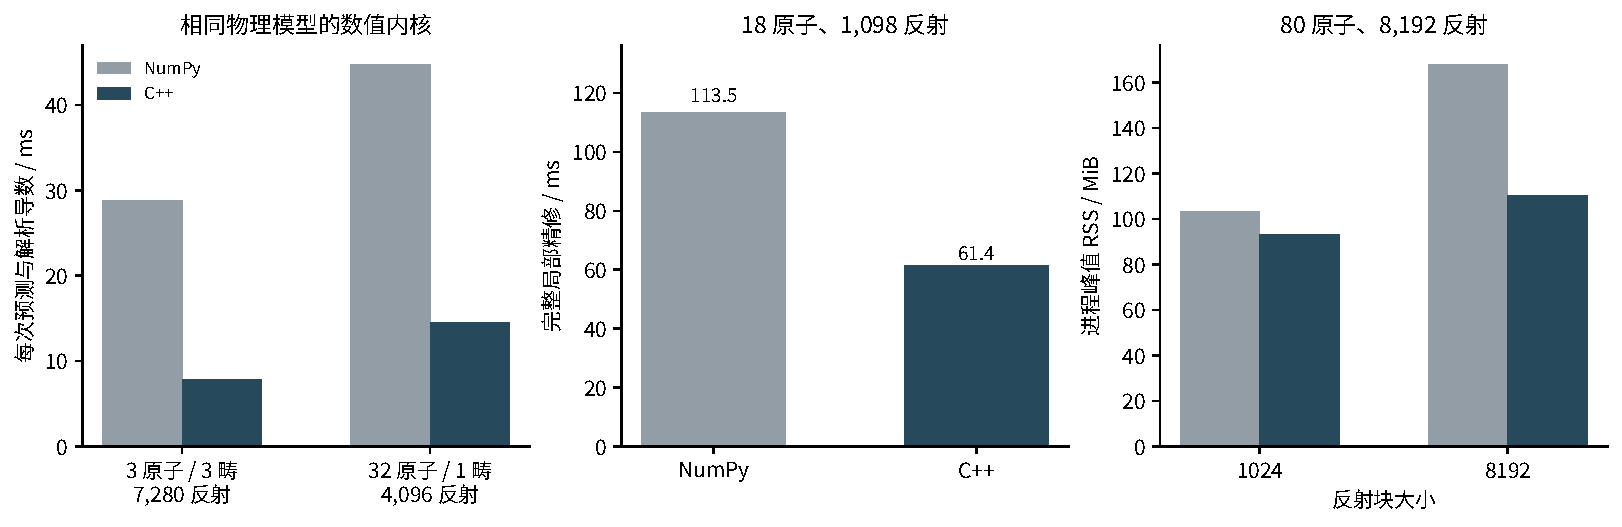
\includegraphics[width=\textwidth]{figures/10_cpp_kernel.pdf}
\caption{可选 C++ 内核的局部实测。左：两种规模的强度及解析 Jacobian，每种后端五轮、每轮八次计算，中位轮时间除以八。中：18 原子完整局部精修的三轮中位时间。右：相同输入的独立进程总峰值 RSS，分别使用两种块长。完整测量及源码摘要保存在 \code{v08_kernel_measurements.json}。}\label{fig:cpp-kernel}
\end{figure}

这组结果支持在重复的结构因子累积处使用融合内核。完整数据还原、FFT 相位检索及任意大型结构的收益需要按各自负载衡量；本章的数值对应明确给出的合成预测问题和已知附近起点的局部精修。发行包同时提供可移植的纯 Python wheel、C++17 源码，以及本平台实编译验证的 CPython 3.12 Linux x86\_64 wheel。
